%% Do not edit unless you really know what you are doing.
\documentclass[twoside,english]{report}

\usepackage[T1]{fontenc}
\usepackage[a4paper]{geometry}
\usepackage[latin9]{inputenc}
\usepackage[sc]{mathpazo}
\usepackage[scaled=0.9]{helvet}
\usepackage{babel}
\usepackage{color}
\usepackage{fancyhdr}
\usepackage{listings}
\usepackage{nomencl}


\geometry{verbose,lmargin=2cm,rmargin=2cm}
\pagestyle{fancy}
\renewcommand{\ttdefault}{lmtt}
\setcounter{secnumdepth}{3}
\setcounter{tocdepth}{3}
\setlength{\parindent}{0pt}
\setlength{\parskip}{\smallskipamount}
\definecolor{llgray}{rgb}{0.9,0.9,0.9}

\newcommand{\code}[1]{\colorbox{llgray}{\lstinline[basicstyle=\ttfamily\color{black}]{#1}}}

% the following is useful when we have the old nomencl.sty package
\providecommand{\printnomenclature}{\printglossary}
\providecommand{\makenomenclature}{\makeglossary}
\makenomenclature
\usepackage[unicode=true,
 bookmarks=true,bookmarksnumbered=false,bookmarksopen=false,
 breaklinks=false,pdfborder={0 0 1},backref=false,colorlinks=false]
 {hyperref}
\usepackage{breakurl}

%%COMMENTARE PRIMA DI PUBBLICARE 
%----------------------------------------------------------------
%\usepackage{draftwatermark} %per il watermark sullo sfondo
%----------------------------------------------------------------
% Per mettere dei commenti per revisione si possono usare i comandi:
% \unsure per le parti in cui non si � sicuri
% \change per le parti che devono essere cambiate in fase di revisone
% \improvement per le parti che devono essere descritte meglio
% \info per scrivere un commento informativo
% \thiswillnotshow � un commento che viene visto solo nel punto in cui viene piazzato e non nella lista delle note
%----------------------------------------------------------------

\makeatletter


% Customization file for the titlepage and document
%************************************************************
% Required stuff
%************************************************************
\usepackage{graphicx}
\usepackage{euler}
\usepackage[detect-all]{siunitx}
\usepackage{sectsty}
\usepackage[font={footnotesize }]{caption}
\usepackage{multicol}
\usepackage{prettyref}

\allsectionsfont{\rmfamily}

% Page customization
\usepackage{fancyhdr}
\pagestyle{fancy}

% Color
\usepackage{color}
\definecolor{light-gray}{gray}{0.85}
\definecolor{dark-gray}{gray}{0.75}

\fancyhead{}  % clear all header fields
\fancyhead[LO,RE]{\rule[-2ex]{0pt}{2ex}\fontsize{9}{11} \selectfont \myPhase}
\fancyhead[RO,LE]{\raisebox{-0.35cm}{
\includegraphics[height=1.2cm,keepaspectratio]{gfx/Logo_TotalBlack.pdf}}}
\fancyhead[CO,CE]{\fontsize{9}{11} \selectfont \myIPT}
\fancyfoot{}  % clear all footer fields
\fancyfoot[RO,LE]{\fontsize{5.5}{8} \selectfont This work is to be considered classified. The use is allowed only for Skyward Experimental Rocketry related activities and projects. For public access please contact \href{mailto:info@skywarder.eu}{info@skywarder.eu}}
\fancyfoot[RE,LO]{\fontsize{9}{11} \selectfont \thepage}
\fancyheadoffset[LE,RO]{0.2pt}
\renewcommand{\headrulewidth}{0.2pt}
\renewcommand{\footrulewidth}{0.2pt}
\renewcommand{\headrule}{\hbox to\headwidth{%
   \leaders\hrule height \headrulewidth\hfill}}
\renewcommand{\footrule}{\hbox to\headwidth{%
    \leaders\hrule height \headrulewidth\hfill}}
\hypersetup{colorlinks=true, linkcolor=blue ,linktoc=page,citecolor=black}

\usepackage{pdfpages} %per includere pdf di più pagine


% Custom notes
\usepackage{xargs}                      % Use more than one optional parameter in a new commands
\usepackage[pdftex,dvipsnames]{xcolor}  % Coloured text etc.

\usepackage[colorinlistoftodos,prependcaption,textsize=tiny]{todonotes}
\newcommandx{\unsure}[2][1=]{\todo[linecolor=red,backgroundcolor=red!25,bordercolor=red,#1]{#2}}
\newcommandx{\change}[2][1=]{\todo[linecolor=blue,backgroundcolor=blue!25,bordercolor=blue,#1]{#2}}
\newcommandx{\info}[2][1=]{\todo[linecolor=OliveGreen,backgroundcolor=OliveGreen!25,bordercolor=OliveGreen,#1]{#2}}
\newcommandx{\improvement}[2][1=]{\todo[linecolor=Plum,backgroundcolor=Plum!25,bordercolor=Plum,#1]{#2}}
\newcommandx{\thiswillnotshow}[2][1=]{\todo[disable,#1]{#2}}
\reversemarginpar
\setlength{\marginparwidth}{2cm}
%End custom notes


%************************************************************
% Redefining numbering for sections
%************************************************************
%\renewcommand*\thesection{\arabic{section}}

%************************************************************
% Cross reference set-up
%************************************************************
\newrefformat{tab}{Table\,\ref{#1}}
\newrefformat{fig}{Figure\,\ref{#1}}
\newrefformat{eq}{Eq.\,\textup{(\ref{#1})}}
\newrefformat{sec}{Sec.\,\ref{#1}}
\newrefformat{sub}{Sec.\,\ref{#1}}

%************************************************************
% Fancy stuff
%************************************************************
\newcommand{\titlecap}[1]{\Huge{\textrm{#1}}}
\newcommand{\subtitlecap}[1]{\Large{\textsc{#1}}}
\newcommand{\sscap}[1]{\textbf{#1}}
\newcommand{\strong}[1]{\textbf{#1}}
\setlength{\headheight}{60pt} %%or

%************************************************************
% Helpful stuff to modify here, not in the LyX Document
%************************************************************
\newcommand{\myDate}{\today}
\newcommand{\myGroup}{Skyward Experimental Rocketry}
\newcommand{\myUrl}{\url{http://www.skywarder.eu}}
\newcommand{\myUni}{Politecnico di Milano}

\newcommand{\myPhase}{Riassunto globale}
\newcommand{\myProject}{Advanced Operating Systems}
\newcommand{\myIPT}{Electronic Systems\\ Integrated Project Team}
\newcommand{\myTitle}{Riassunto}
\newcommand{\myAuthor}{Matteso}
\newcommand{\myEditor}{Nobody}
\newcommand{\myEmail}{XX@skywarder.eu}

\newcommand{\mail}[1]{\href{mailto:#1}{\texttt{#1}}}

\makeatother

\begin{document}
\thispagestyle{empty}
\pdfbookmark{Titlepage}{Titlepage}

\vspace{3cm}
\begin{center}
\bigskip
\Large{\myDate}
\vspace{0.5cm}

{\titlecap{Project \myProject} \\
\vspace{0.3cm}
\titlecap{\myPhase}}\\
\vspace{0.4cm}
\rule{\linewidth}{0.5mm}
\titlecap{\myTitle}
\end{center}

\vfill
\begin{multicols}{2}
\centering{

\includegraphics[height=4cm]{gfx/Logo_Colour.pdf} \\

\includegraphics[height=3cm]{gfx/Logo_Polimi}
}
\vfill
\columnbreak
{\centering{
	\subtitlecap{\myIPT} \\
	\vspace{0.7em}
	\normalsize
	\textrm{\myGroup \\
	\myUni }}}
\vfill

\raggedright{\textbf{Author}: {\myAuthor}\\
\textbf{Editor}: {\myEditor}}

						
\end{multicols}

\clearpage

%*******************************************************
% Titleback
%*******************************************************
\thispagestyle{empty}

\hfill
\vspace{5cm}

\strong{Abstract}\\
Scrivi qui il tuo abstract
\vfill

\begin{multicols}{2}
\medskip
\noindent{\sscap{Website}}: \\
\url{http://www.skywarder.eu}


\medskip
\noindent{\sscap{E-mail}}: \\
\mail{\myEmail}
\vfill
\columnbreak
\section*{Restricted use policy}
\fontsize{8}{11} \selectfont This report is developed during the activities done within Skyward Experimental Rocketry association. Its use is allowed only for Skyward Experimental Rocketry related purposes. If you're a Skyward member, please don't send or release publicly this file without previous acceptance from Direction Board.
For public access and publication please contact \href{mailto:info@skywarder.eu}{info@skywarder.eu}.
\end{multicols}
\vspace{1cm}
\hrule
\bigskip
\clearpage


\pagenumbering{roman}

\begin{multicols}{2}

\printnomenclature{}

\end{multicols}

\tableofcontents{}

\listoffigures


\listoftables

%%COMMENTARE PRIMA DI PUBBLICARE 
%----------------------------------------------------------------
\listoftodos[Notes] %per avere l'elenco delle note
%----------------------------------------------------------------

\clearpage{}

\pagenumbering{arabic}

\setcounter{page}{1}

\global\long\def\diff{\text{d}}



\chapter{Git}
\section{Initialize repository}
\begin{itemize}
\item \code{git init .}, initialize a new repository in the current folder 
\item \code{git clone <repository url>} downloads a full remote repository to the local computer, but has to be done on an empty folder.
\end{itemize}

\section{Work with GIT}
\begin{itemize}
\item \code{git add <files>}, add some files to the staging area.  with "." add every file in the folder, "*.tex" just the \LaTeX  files.
\item \code{git status}, show the status of the repo (added files, untracked files, etc.
\item \code{git log}, gives information about all the commits of the repository, with each comment.
\item \code{git commit -m "message"}, Commits locally the changes. Files marked as ``to-be-committed`` using \code{git add} or \code{git rm} commands will be ''stored`` in the internal database. The commit description is specified with the \textbf{-m} param.
\item \code{git commit -am "message"}, commits all changed files (it's like a \\ \code{git add . \&\& git commit -m "message"}, using the specified message as commit description.
\\ \code{git reset HEAD <nome\ file>} to remove a file from the staging area 
\end{itemize}

\section{Remote repository management}
\begin{itemize}
\item \code{git fetch <repository name>}, update just the ``header'' of the repo, which contains the list of branches and so on.
\item \code{git remote add <repo name> <repo url>}, specify a remote repo url that will be used with \code{git push} or \code{git pull} commands. 
\item \code{git push -u <repo name> <branch name>} upload the changes to \code{repo_name} in the branch \code{branch_name}. \code{-u} means that (in future) typing \code{git push} will always use this host and branch.
\item \code{git pull <repo name> <branch name>} download the changes from the branch \code{branch_name} on \code{repo_name}. If the remote repo is stored as default (or it's the only one), \code{git pull} will work as well.
\end {itemize}

\section{Branch}
\subsection{Create a new Branch}
\begin{itemize}
\item \code{git checkout -b <new branch name>}
\item \code{git add <file to commit>}
\item \code{git commit -m "comment"}
\item \code{git push -u <repo name> <new branch name>}
\end{itemize}

\subsection{Merge Branch with master}
\begin{itemize}
\item \code{git checkout master}, move to the master branch (or whatever branch you want to merge with).
\item \code{git merge <branch name>}, merges the specified branch with the actual branch.
\end{itemize}

\subsection{Switch to an other branch}
\begin{itemize}
\item \code{git checkout <branch name>}
\end{itemize}

\section{Undo Commands}
\begin{itemize}
\item \code{git reset --soft}, unstage committed files
\item \code{git reset --hard}, delete changes to the last commit
\item \code{git commit --amend}, change last commit
\item \code{git revert <SHA-1 commit id>}, revert to a specific commit
\end{itemize}

Just a note, \code{git commit --amend} will change the whole GIT tree. So, 
if the commit is already uploaded on  the server, a \code{git push -f} will be
required.  \code{git push -f} is the second name of Satan. Be aware that
after that there will be high chances to destroy the whole GIT tree, losing
everything. Hence, \code{git commit --amend} is bad.

\section{Useful links}
\begin{itemize}
\item \url{https://try.github.com}
\end{itemize}

\begin{figure}[h]
	\centering
	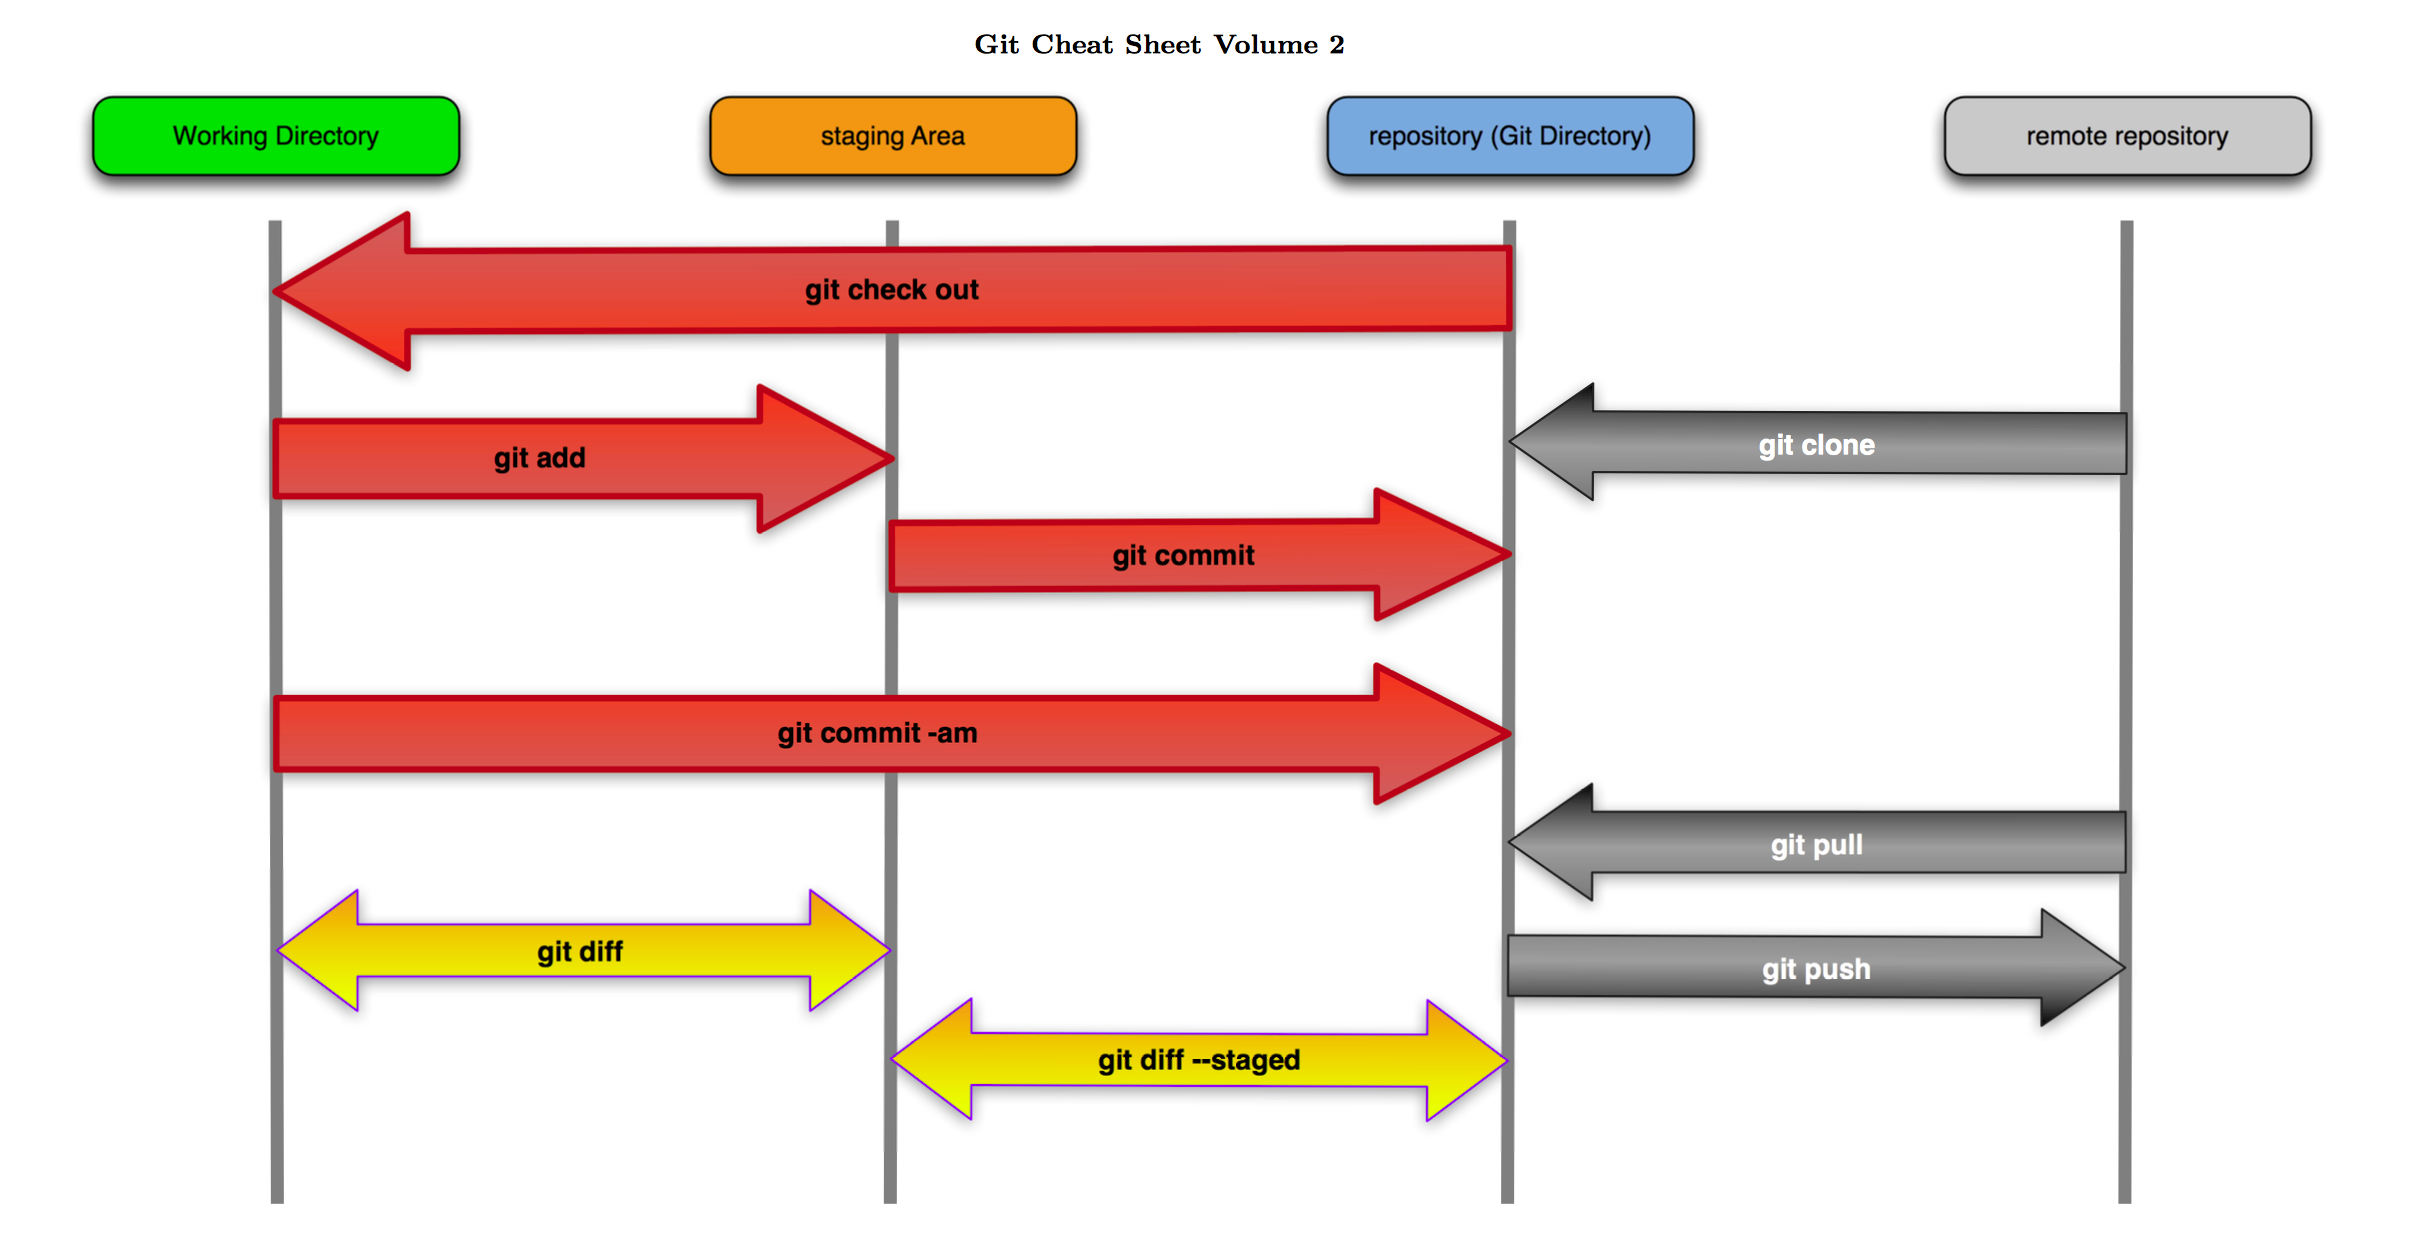
\includegraphics[width=\textwidth]{gfx/git_graph}
	
	\caption{Comandi GIT}
	\label{Fig:Commands}
\end{figure}


\chapter{Scheduling}
\section{Criteria}
Algorithms can be optimized for different goals:
\begin{itemize}
\item \textbf{CPU utilization}, keep CPU as busy as possible
\item \textbf{throughput}, number of processes that complete their execution per time unit
\item \textbf{turnaround time}, amount of time to execute a particular process
\item \textbf{waiting time}, amount of time a process has been waiting in the ready queue
\item \textbf{response time}, amount of time it takes from when a request was submitted until the first response is produce, not output

\end{itemize}

\section{Algorithms}
A detailed description is provided in Table \ref{Tab:Algorithms}.
\begin{table}[]
	\centering
	\resizebox{\textwidth/8*7}{!}{%
		\begin{tabular}{|m{\textwidth/11}|m{\textwidth/10}|m{\textwidth/11}|m{\textwidth/11}|m{\textwidth/9}|m{\textwidth/9}|m{\textwidth/9}|m{\textwidth/11}|m{\textwidth/7}|m{\textwidth/9}|m{\textwidth/8}|}
			\hline
			\textbf{Scheduler}                   & \textbf{Preemptive} & \textbf{Priority} & \textbf{CPU Utilization} & \textbf{Thrughput} & \textbf{Turnaround time}                             & \textbf{Waiting time}                           & \textbf{Response time}                          & \textbf{Advantages}                                                                                                                    & \textbf{Issues}                                                                                         & \textbf{Description}                                                                                                       \\ \hline
			First Come First Served (FCFS)       & NO                  & NO                & LOW                      & LOW                & SHORTEST                                             & HIGH                                            & HIGH                                            & Semplicity                                                                                                                             & Processes may starve if after long process                                                              & Favours CPU-bound processes                                                                                                \\ \hline
			Shortest Job First (SJF)             & NO                  & NO                & HIGH                     & HIGH               & LONG for long processes, SHORTEST for fast processes & HIGH for long processes, LOW for fast processes & HIGH for long processes, LOW for fast processes & Minimum Average Waiting time                                                                                                           & Long processes may starve, must estimate process time: not implementable in most cases for this reason. & Favours the processes that need less CPU-time                                                                              \\ \hline
			Shortest Remaining Time First (SRTF) & YES                 & NO                & HIGH                     & HIGH               & LONG for long processes, SHORTEST for fast processes & MEDIUM                                          & MEDIUM                                          & If a shorter task is available, it runs immediately in CPU, less overhead (the scheduler decides only when another process approaches) & Long processes may starve (worst than SJF), must estimate process time.                                 & It's the SJF but with preemption                                                                                           \\ \hline
			Higher Response Ratio Next           & NO                  & YES               & HIGH                     & MEDIUM             & MEDIUM                                               & LOW                                             & MEDIUM                                          & Prevents starvation by assigning higher priority to processes waiting for a long time.                                                 & must estimate process time                                                                              & It's the evolution of SJF.                                                                                                 \\ \hline
			Feedback                             & YES                 & NO                & HIGH                     & LOW                & LONG                                                 & LOW                                             & LOW                                             & No starving processes, don't know remaining time process needs to execute.                                                             & High overhead and continuous context switch                                                             & Penalizes jobs that have been runnning longer                                                                              \\ \hline
			Fair-Share Scheduling (FSS)          & YES                 & NO                & LOW                      & LOW                & LONG                                                 & LOW                                             & LOW                                             & Every process has its fair share of CPU time, useful with multiple group users.                                                        & Processes in crowded groups get less CPU time                                                           & Applies the round-robin scheduling strategy at each level of abstraction (processes, users, groups, etc.)                  \\ \hline
			Round Robin                          & YES                 & NO                & HIGH                     & MEDIUM             & LONG                                                 & LOW                                             & LOW                                             & No starvation, equal waiting time                                                                                                      & Longer turnaround time (every process takes longer if slower than a time quantum)                       & Uses preemption based on a clock, every process is executed in 1 time quantum and than leaves the CPU to the next process. \\ \hline
		\end{tabular}%
	}
	\caption{Main Scheduling Algorithms}
	\label{Tab:Algorithms}
\end{table}

\pagebreak

\section{Multilevel Queue}
\begin{itemize}
	\item{\textbf{multilevel queue}}, the scheduler select the queue for a process according to its type. Process does not change its queue
	\item{\textbf{multilevel feedback queue}}, process starts in the first queue but if do not complete after the first execution scheduler in the next queue
\end{itemize}

\section{Multiprocessor Scheduling}
\begin{table}[h]
	\centering

	\begin{tabular}{|m{\textwidth/15}|m{\textwidth/6}|m{\textwidth/6}|m{\textwidth/6}|m{\textwidth/6}|}
		\hline
		& \textbf{COMPLEXITY} & \textbf{OVERHEAD} & CPU UTILIZATION & ISSUES \\ \hline
		\textbf{MASTER/ SLAVE} & LOW, there is a master processor that manage the ready process queue and the common resources & LOW, static assignament of process there are few content switch & LOW, a low demanding task can lock a cpu & the master core is the bottle neck of the system\\ \hline
		
		\textbf{PEER} & HIGH, every processor has its own scheduler that have to race for common resources & HIGH, the same process can start in a processor and then jump to another & HIGH &high complexity in shared resources management \\ \hline
		
	\end{tabular}
	\caption{Multiprocessing scheduling characteristics}
	\label{tab:multiprocessing}
\end{table}

\section{Content Switch}
is a particular state of OS in which the current process in execution is stopped, the context (value of the program counter and of the register) is saved in PCB (process control bock) to allow to conitnue the execution on the future and is set the context of the new process selected from the ready queue by the scheduler.\\
\textbf{When it occours:} \\
\begin{itemize}
		\item in multitasking execution
		\item when an interrupt occours
		\item switching from kernel mode to user mode (in some architectures the cost of this operation can be lower than the other two cases)
\end{itemize}
\textbf{hardware implementation:} \\
a content switch can be implemented \underline{explicitly} with a CALL or JMP instruction to the TSS (task state segment) in global descriptor table\\
or \underline{implicitly} by hardware support that when an interrupt occours automatically save the context in special shadow registers and execute the task according to the interrupt descriptor table.\\
Sometime there can be some limitation to the hardware approach that depends from the archiecture, for example in some case the registers used by the task can be different from the general pourpose regiser of shadow reg and a software approach would be better.









\chapter{RTOS}
\section{Types}
There are two types of RTOS:
\begin{itemize}
	\item \textbf{Hard real-time}: timing violation is not accettable (car, ecc..)
	\item \textbf{Soft real-time}: timing violation is undesiderable but accettable (video, music, ecc..)
\end{itemize}

\section{Features}
The main features of an RTOS are:
\begin{itemize}
	\item \textbf{Determinism}: operation are performed at fixed and predetermined times \textbf{or} within predetermined time intervals. It defines how much time it takes to react, but \textbf{not} to complete the operation (i.e. how long does it take to handle and interrupt).
	\item \textbf{Resposiveness}: how long, after acknowledgement, the operating system takes to \textbf{service} (complete) the task (i.e. the interrupt). It depends on ISR nesting.
	\item \textbf{Reliability}: degradation of performances should not impact the system:	
	\begin{itemize}
		\item Fail soft: Ability to fail in such a way to preserve as much data
		\item Stability: the system adopts policies such that the most critical high priority tasks execute first, even if some needs of less important tasks cannot be met.
	\end{itemize}
\end{itemize}




\section{Algorithms}
%\begin{itemize}
%	\item \textbf{static-table driven}	
%	
%	
%	\item \textbf{dynamic-best effort}
%	\item \textbf{}
%\end{itemize}\
	
\begin{table}[]
	\centering
	\resizebox{\textwidth*9/10}{!}{%
		\begin{tabular}[\scriptsize]{|m{\textwidth/10}|m{\textwidth/10}|m{\textwidth/10}|m{\textwidth/10}|m{\textwidth/10}|m{\textwidth/10}|}
			\hline
			\textbf{Algorithm} & \textbf{Online Schedulability analysis} & \textbf{Static/Dynamic} & \textbf{Advantages} & \textbf{Issues} & \textbf{Description} \\ \hline
			
			\textbf{Static-Table Driven, (Time triggered system)} & NO. & STATIC & Easy to implement & the system can't manage tasks that aren't in the TDL & Sync of process and dependencies are saved in a TDL (Task Descriptor List). At every clock process are executed according to this table \\ \hline
			
			\textbf{Dynamic Best Effort (Earliest Deadline First)} & NO. Offline the condition is $\sum \frac{C_i}{T_i} < 1$  & DYNAMIC & Easy, no analysis of schedulability and only a condition $\sum \frac{C_i}{T_i} \le 1$. Ideal for periodic tasks & Executing a task that could not meet the deadline may prevent other tasks to reach their deadlines and the number of tasks that will miss the deadline is unpredictable. & Through a static analysis of the tasks determines, at run time, when a task has to be executed (applicable to periodic tasks). The system tries to meet dedlines and aborts any started process whose deadline is missed. Until the task is completed or the deadline arrives, it is unknown if time constraints will be met. \\ \hline
			
			\textbf{Rate Monotonic} & NO. The offline condition of schedulability is $\sum \frac{C_i}{T_i} < n(2^{\frac{1}{n}}-1)$ there is a upper limit 69 percent  & STATIC & Simpler than EDF, if the formula is valid, ensures we will never miss a deadline. & It's not always possible to achieve maximum CPU utilization & Every task has a priority, shortest period task highest priority and therefore is executed first. \\ \hline
			
			\textbf{Dynamic Planning Based} & YES & DYNAMIC & A task is accepted for execution if and only if is feasible to meet its time constraints & Quite complicate to implement & Before a task execution an attempt is made to create a schedule including previous tasks and the new one. \\ \hline
			
		\end{tabular}%
	}
	\caption{RTOS algorithms}
	\label{tab:RTOS_algs}
\end{table}





\begin{table}[]
	\centering
	\resizebox{\textwidth}{!}{%
		\begin{tabular}{|m{\textwidth/20}|m{\textwidth/6}|m{\textwidth/6}|m{\textwidth/6}|}
			\hline
			& \textbf{COMPLEXITY} & \textbf{CPU UTILIZATION} & \textbf{DEADLINE} \\ \hline
			\textbf{RMS} & \textbf{LOW}, the priority is fixed, set by T & MEDIUM, all tasks have dead time $\sum{\frac{C_i}{T_i}} \le N(N^{\frac{1}{N}}-1)$ (max lim $\rightarrow \infty$), max 69\% & hi P process met deadline everytime \\ \hline
			\textbf{EDF} & HIGH, real time raise priority to task with earlier deadline & HIGH, process are preempted continuously $sum{\frac{C_i}{T_i}} \le 1$, (max 100\%) & if system is overloaded the set of process that fail deadline are large and unpredictable \\ \hline
		\end{tabular}%
	}
	\caption{RTOS Scheduling Algorithms}
	\label{tab: RTOS_schedulingl}
\end{table}


\chapter{RT scheduling}

\section {cyclic scheduling}
\section{deterministic scheduling}
\section{capacity-based scheduling}
\section{dynamic priority scheduling}
\section{Scheduling Task with imprecise Results}



\chapter{Linux App Dev}
\section{Building process}
As seen from Figure \ref{Fig:Build_process}, the building process is composed by various phases:
\begin{itemize}
	\item Using an editor, you create the source and header files.
	\item The makefile defines which operations are needed to complete the build and which files have to be build.
	\item The preprocessor analyzes the source code and runs the preprocessor directives: macros, \#defines, ecc.. are expanded in "normal code": the full source is now ready to be compiled and goes in one *.i file. This operation can be seen by stopping the building process with the command \code{g++ -E main.c -o hello.i}
	\item After compiling the *.i files we get the assembly code, another human-readable text file. This output file can be seen by stopping the building process with the command \code{g++ -c hello.c}
	\item The next step is assembling the code: an *.o (object) file is generated, that's something really close the machine code, but still not hardware dependent: the memory addresses are still relative and the library calls are still not included.
	\item The final step is linking: it adds the static libraries to the code and generates the final executable file.
\end{itemize}
\begin{figure}[h]
	\centering
	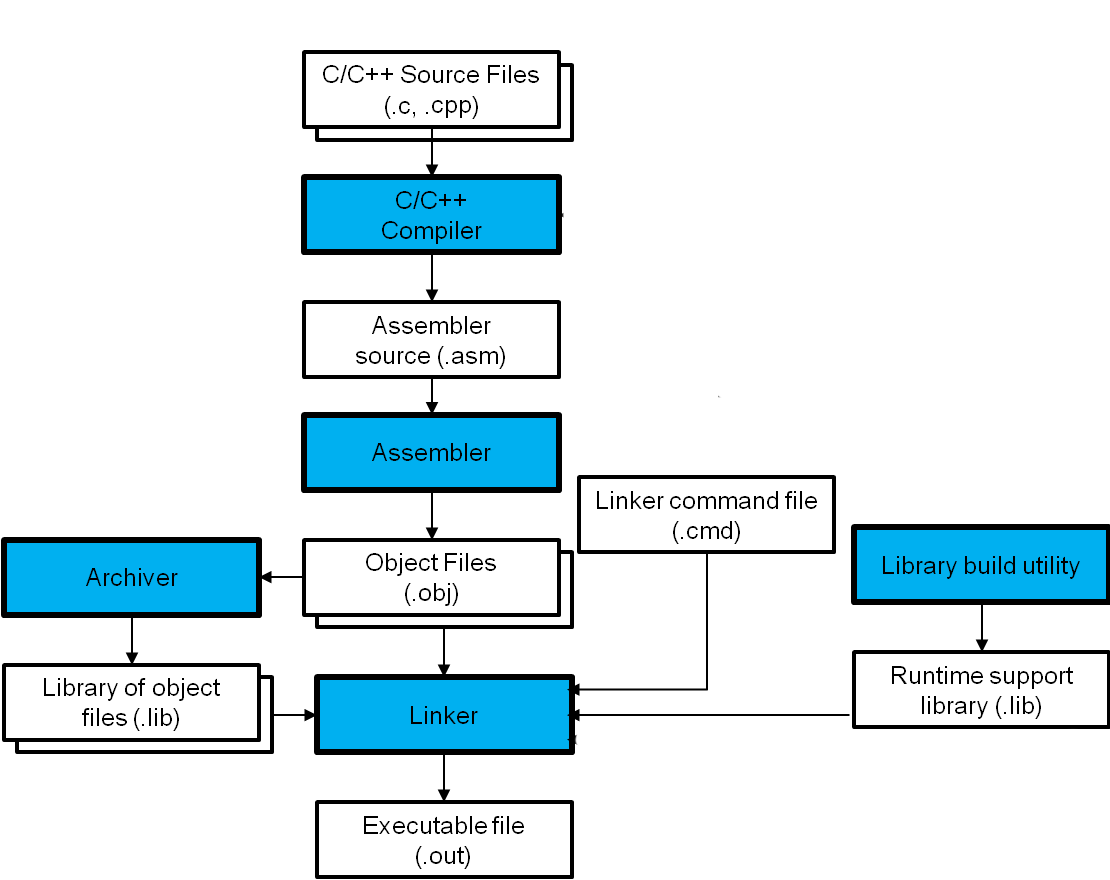
\includegraphics[width=\textwidth]{gfx/build_process}
	
	\caption{Build Process Procedure}
	\label{Fig:Build_process}
\end{figure}

\section{Makefile}
TODO

\section{Linker Script}
The linker script is a file that defines where the various parts of the compiled code are actually stored in memory.

The simplest possible linker script has just one command:\code[SECTIONS]. This command describes the memory layout of the building output file.

Let's assume that the program consists only of code, initialized data and uninitialized data: these will be, respectively, stored in the \code[.text], \code{.data} and \code{.bss} sections.

The linker script that could place these section in the correct parts of the memory would be something like:


\begin{figure}[h]
	\centering
	
\includegraphics[width=\textwidth/3]{gfx/linker_file}
	
	\caption{Linker file example}
	\label{Fig:Linker File}
\end{figure}



\chapter{Exam Questions}
\section{First question -----}

\chapter{Hardware Exercice}
\section{bit operation}
\begin{itemize}
	\item left shift operator \code{(1<<2)} = 0b0100
	\item setting 1a precise bit keeping unchanged the others for exampe 0b0000 $\rightarrow$ 0b0100 \\
	0b0000 = 0b0000 | 0b0100; \\
	that is the same of
	0b0000 |= 0b0100; 
	

	\item setting 0 to a precise bit\\
		ex: 0b1111 $\rightarrow$ 0b1011 \\ 0b1111 \&= 0b1011; \\0b1111 $\&$= \code{(2<<0)}
		
	\item check if a bit is 1 \\ 
	ex: if(0b0010 $\&$ 0b0010) $==$ 1   VERO \\	
	ex: if(0b0010 $\&$ 0b0001) $==$ 1   FALSO
	
	\item check if a bit is 0 \\
	ex: if(0b1101 | $\sim$(0b0010)) $==$ 0  VERO \\	
	ex: if(0b1111 | $\sim$(0b0010)) $==$ 0   FALSO \\	

	\end{itemize}

\section{access register}
\subsection{method 1: every variable a register}
declare a variable volatile unisgned with the size of the desired register\\
\begin{lstlisting}
/*ex: 8bit register @ address 0x03AA*/ \\
$($volatile unsigned char$*)$ register $=$ 0x03AA$;$ \\
\end{lstlisting}


\subsection{method 2: struct}
struct REG_Struct${$ \\
volatile unsigned char reg1$;$ \\
unsigend char padding$[3];$ \\
volatile unsigned short reg2$;$ \\
$};$ \\

$\#$define (struct REG_Struct $*$) $<$address$>$





%inserire un PDF nel pdf
%\begin{figure}[h]
%	\centering
%	\includegraphics[scale=1]{doc/nome_del_documento}
%	
%	\caption{descrizione, se necessaria}
%	\label{Fig:etichetta_documento}
%\end{figure}

\end{document}
